\documentclass[12pt]{article}

\usepackage[a4paper,margin=1in]{geometry}
\usepackage{setspace}
\onehalfspacing

\usepackage{amsmath,amssymb,amsthm}
\usepackage{graphicx}
\usepackage{float}
\usepackage{caption}
\usepackage{subcaption}
\usepackage{enumitem}
\usepackage{makecell}

% \begin{figure}[htbp]
%     \centering
%     
\includegraphics[width=0.6\textwidth]{hw1_q2b_surface.png}
%     \caption{Optimal joint density f(p, d)}
%     \label{fig:2b}
% \end{figure}

\title{ECON 5345 Homework 5 Report}
\author{Harlly Zhou}
\date{\today}

\begin{document}

\maketitle

\begin{enumerate}[label=\arabic*.]
   \item The following table reports the results of the lag selection. The AIC chooses $p=6$, the BIC chooses $p=1$, and the likelihood ratio test chooses $p=3$ (We reject $p=4$ at the 5\% significance level).
   \begin{table}[!htbp]
    \centering
    \caption{Lag selection statistics for the VAR model}
    \begin{tabular}{cccc}
    \hline
    $p$ & AIC & BIC & LR $p$-value \\
    \hline
    1 & -1.456476 & -1.026065 & 0.0157 \\
    2 & -1.445090 & -0.670350 & 0.0000 \\
    3 & -1.609263 & -0.490194 & 0.0005 \\
    4 & -1.680275 & -0.216877 & 0.0536 \\
    5 & -1.636079 & 0.171648  & 0.0004 \\
    6 & -1.710671 & 0.441384  & 0.1895 \\
    7 & -1.627121 & 0.869263  & 0.0036 \\
    8 & -1.651718 & 1.188995  & -- \\
    \hline
    \end{tabular}
    \label{tab:var_lag_selection}
    \end{table}

    \newpage
    \item The following table reports the least squares estimates of the $VAR(6)$ model. Each cell reports the coefficient with significance stars and the $t$-statistic in parentheses.
    \begin{table}[htbp]
        \centering
        \caption{VAR(6) least squares estimates. }
        \label{tab:hw5_q2_var_ols}
        \scriptsize
        \begin{tabular}{lcccc}
        \hline
        RHS regressor & $\Delta\log(\text{Real GDP})$ & $\Delta\log(\text{GDP Deflator})$ & $\Delta\log(\text{EXR})$ & FFR \\
        \hline
        
        Constant 
        & \makecell{0.2803\\(1.145)}
        & \makecell{-0.0043\\(-0.059)}
        & \makecell{-0.7676\\(-0.738)}
        & \makecell{-0.6635*\\(-2.221)} \\
        
        $\Delta\log(\text{Real GDP})_{t-1}$
        & \makecell{0.3590***\\(3.496)}
        & \makecell{0.0218\\(0.705)}
        & \makecell{-0.1342\\(-0.307)}
        & \makecell{0.4713***\\(3.761)} \\
        
        $\Delta\log(\text{GDP Deflator})_{t-1}$
        & \makecell{-0.5061.\\(-1.669)}
        & \makecell{0.5533***\\(6.055)}
        & \makecell{-1.0817\\(-0.840)}
        & \makecell{-0.2412\\(-0.652)} \\
        
        $\Delta\log(\text{EXR})_{t-1}$
        & \makecell{0.0027\\(0.114)}
        & \makecell{-0.0134.\\(-1.895)}
        & \makecell{0.3885***\\(3.895)}
        & \makecell{-0.0347\\(-1.211)} \\
        
        $FFR_{t-1}$
        & \makecell{0.1120\\(1.420)}
        & \makecell{0.0766**\\(3.223)}
        & \makecell{-0.0502\\(-0.150)}
        & \makecell{1.0867***\\(11.291)} \\
        
        $\Delta\log(\text{Real GDP})_{t-2}$
        & \makecell{0.1610\\(1.467)}
        & \makecell{-0.0690*\\(-2.086)}
        & \makecell{-0.5039\\(-1.080)}
        & \makecell{0.2789*\\(2.082)} \\
        
        $\Delta\log(\text{GDP Deflator})_{t-2}$
        & \makecell{1.4582***\\(4.169)}
        & \makecell{0.1695\\(1.608)}
        & \makecell{1.4276\\(0.960)}
        & \makecell{1.3122**\\(3.074)} \\
        
        $\Delta\log(\text{EXR})_{t-2}$
        & \makecell{-0.0191\\(-0.759)}
        & \makecell{-0.0049\\(-0.640)}
        & \makecell{-0.1293\\(-1.207)}
        & \makecell{-0.0221\\(-0.718)} \\
        
        $FFR_{t-2}$
        & \makecell{-0.4387***\\(-3.861)}
        & \makecell{-0.0796*\\(-2.323)}
        & \makecell{0.0062\\(0.013)}
        & \makecell{-0.4988***\\(-3.597)} \\
        
        $\Delta\log(\text{Real GDP})_{t-3}$
        & \makecell{-0.0752\\(-0.649)}
        & \makecell{0.0352\\(1.006)}
        & \makecell{1.1853*\\(2.406)}
        & \makecell{0.1018\\(0.719)} \\
        
        $\Delta\log(\text{GDP Deflator})_{t-3}$
        & \makecell{-0.9872**\\(-2.707)}
        & \makecell{-0.0423\\(-0.384)}
        & \makecell{-1.4989\\(-0.967)}
        & \makecell{-0.6605\\(-1.484)} \\
        
        $\Delta\log(\text{EXR})_{t-3}$
        & \makecell{0.0308\\(1.252)}
        & \makecell{-0.0044\\(-0.595)}
        & \makecell{0.1781.\\(1.706)}
        & \makecell{-0.0139\\(-0.463)} \\
        
        $FFR_{t-3}$
        & \makecell{0.2735*\\(2.289)}
        & \makecell{0.0273\\(0.759)}
        & \makecell{-0.0169\\(-0.033)}
        & \makecell{0.5663***\\(3.883)} \\
        
        $\Delta\log(\text{Real GDP})_{t-4}$
        & \makecell{0.1806.\\(1.711)}
        & \makecell{0.0868**\\(2.726)}
        & \makecell{-0.0549\\(-0.122)}
        & \makecell{-0.1657\\(-1.286)} \\
        
        $\Delta\log(\text{GDP Deflator})_{t-4}$
        & \makecell{0.0639\\(0.171)}
        & \makecell{0.3038**\\(2.698)}
        & \makecell{2.6168\\(1.648)}
        & \makecell{-0.4141\\(-0.908)} \\
        
        $\Delta\log(\text{EXR})_{t-4}$
        & \makecell{-0.0097\\(-0.400)}
        & \makecell{-0.0011\\(-0.151)}
        & \makecell{-0.0770\\(-0.749)}
        & \makecell{0.0106\\(0.360)} \\
        
        $FFR_{t-4}$
        & \makecell{-0.0054\\(-0.045)}
        & \makecell{-0.0628.\\(-1.727)}
        & \makecell{-0.5041\\(-0.983)}
        & \makecell{-0.2130\\(-1.446)} \\
        
        $\Delta\log(\text{Real GDP})_{t-5}$
        & \makecell{0.0896\\(0.890)}
        & \makecell{0.0179\\(0.589)}
        & \makecell{-0.5004\\(-1.170)}
        & \makecell{0.1938\\(1.578)} \\
        
        $\Delta\log(\text{GDP Deflator})_{t-5}$
        & \makecell{0.6285\\(1.601)}
        & \makecell{-0.1428\\(-1.207)}
        & \makecell{-3.3585*\\(-2.013)}
        & \makecell{0.0800\\(0.167)} \\
        
        $\Delta\log(\text{EXR})_{t-5}$
        & \makecell{-0.0030\\(-0.126)}
        & \makecell{-0.0073\\(-1.004)}
        & \makecell{-0.0830\\(-0.813)}
        & \makecell{-0.0472\\(-1.611)} \\
        
        $FFR_{t-5}$
        & \makecell{-0.0774\\(-0.649)}
        & \makecell{0.0781*\\(2.174)}
        & \makecell{1.5854**\\(3.130)}
        & \makecell{0.3486*\\(2.396)} \\
        
        $\Delta\log(\text{Real GDP})_{t-6}$
        & \makecell{-0.1052\\(-1.131)}
        & \makecell{-0.0343\\(-1.224)}
        & \makecell{0.1793\\(0.454)}
        & \makecell{-0.0700\\(-0.616)} \\
        
        $\Delta\log(\text{GDP Deflator})_{t-6}$
        & \makecell{-0.5657.\\(-1.779)}
        & \makecell{0.1020\\(1.064)}
        & \makecell{2.1000\\(1.554)}
        & \makecell{0.3177\\(0.819)} \\
        
        $\Delta\log(\text{EXR})_{t-6}$
        & \makecell{0.0232\\(0.984)}
        & \makecell{0.0013\\(0.179)}
        & \makecell{-0.0010\\(-0.010)}
        & \makecell{0.0113\\(0.392)} \\
        
        $FFR_{t-6}$
        & \makecell{0.1217\\(1.447)}
        & \makecell{-0.0421.\\(-1.662)}
        & \makecell{-0.9697**\\(-2.713)}
        & \makecell{-0.3526***\\(-3.436)} \\
        
        \hline
        \end{tabular}
        
        \vspace{0.4em}
        \footnotesize
        Signif. codes: *** $p<0.01$, ** $p<0.05$, * $p<0.1$, . $p<0.1$.
        $t$-statistics in parentheses.
        \end{table}

    \newpage
    \item The following figure reports the IRF together with the error bands with parametric MC and bootstrap.
    \begin{figure}[htbp]
        \centering
        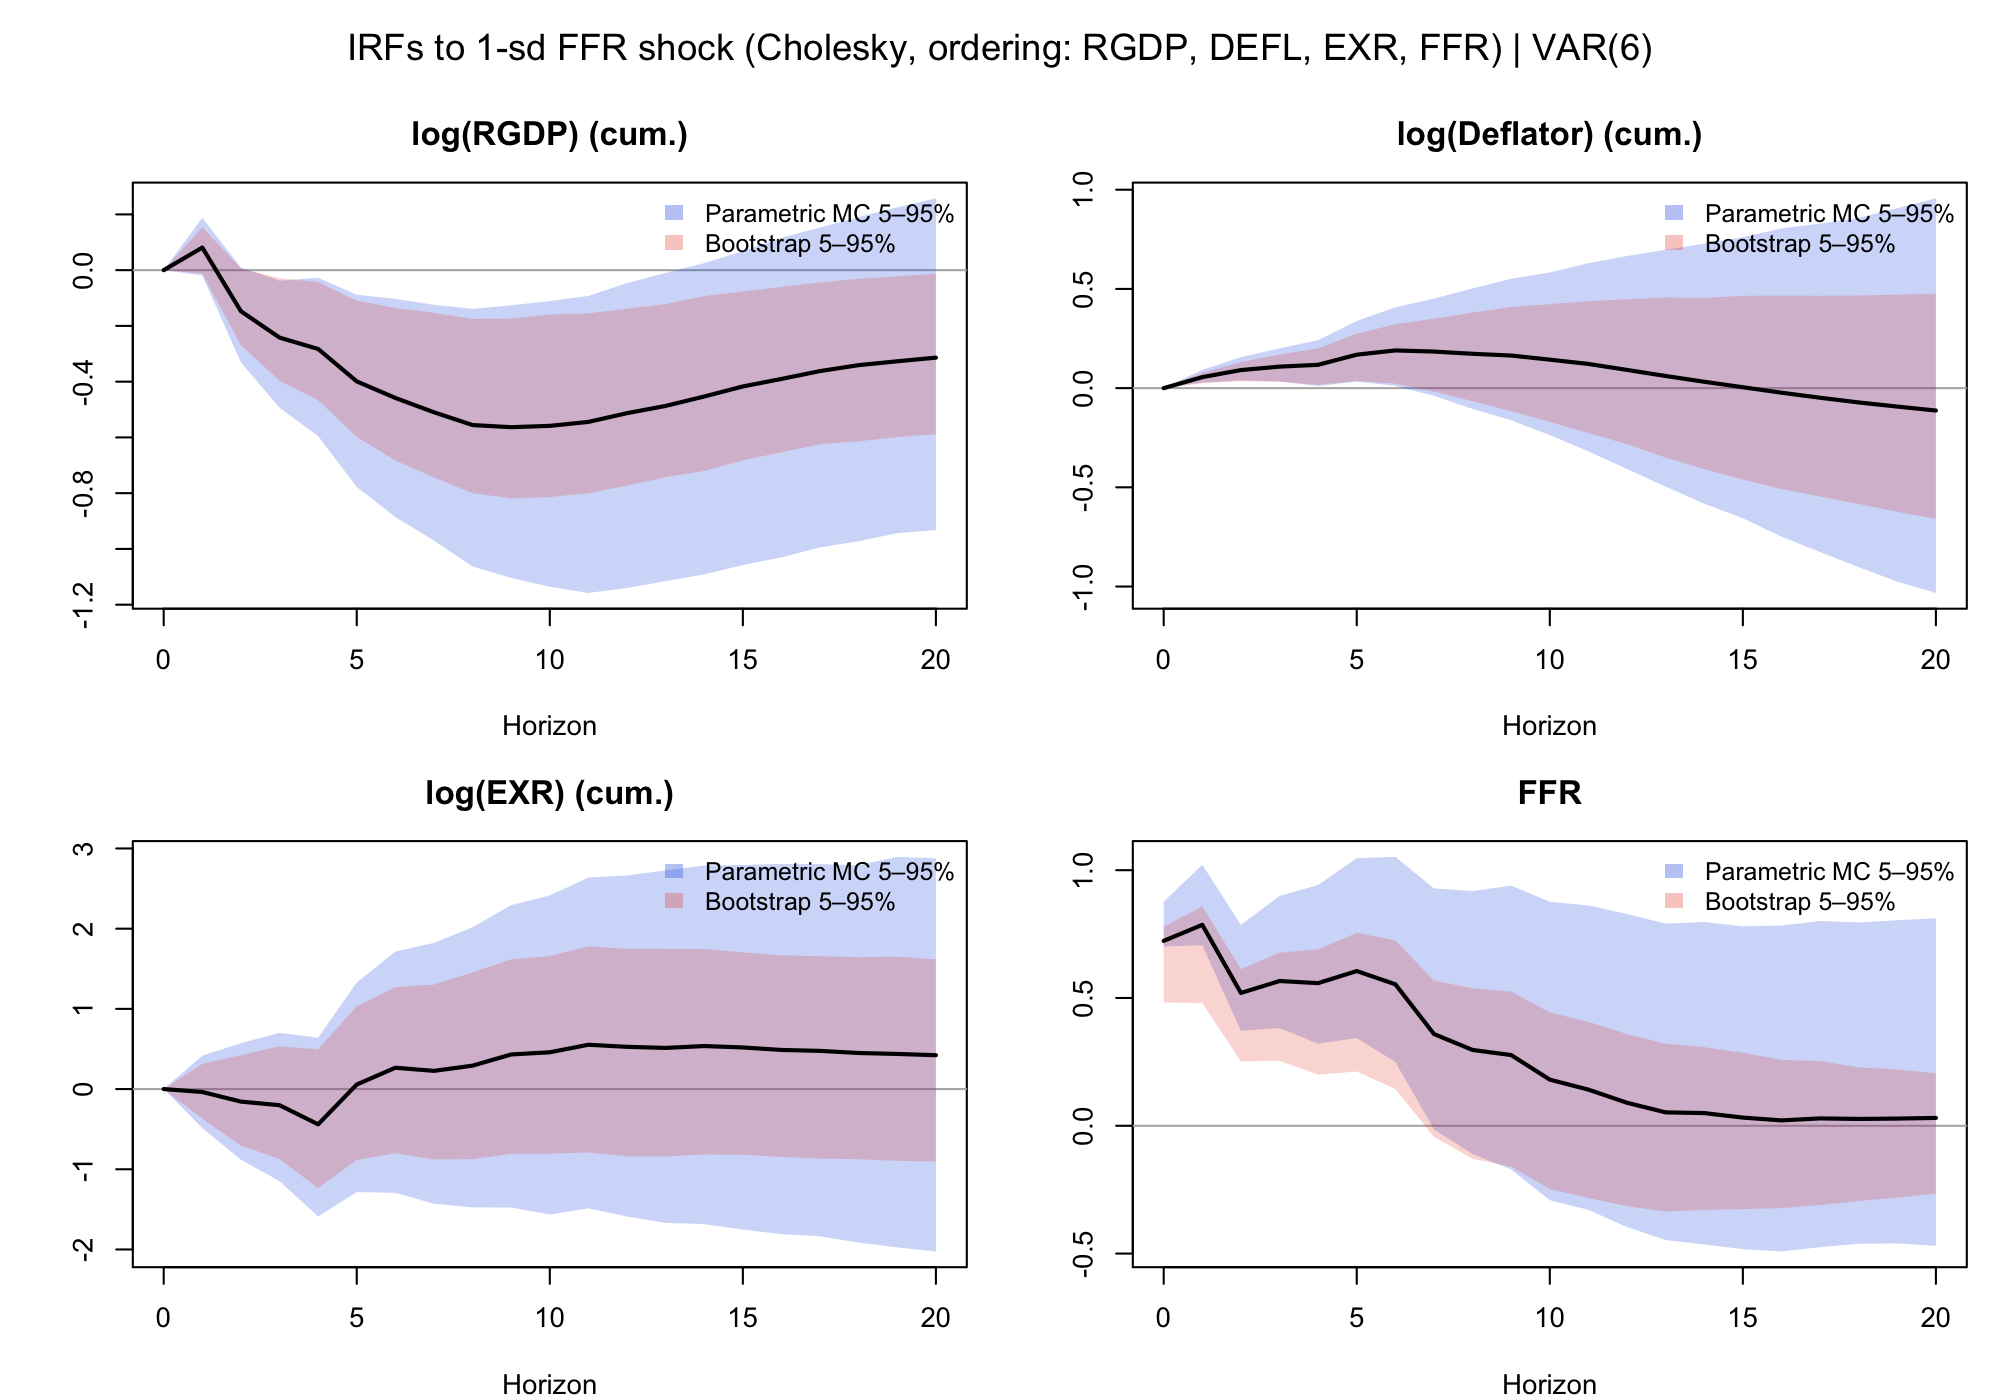
\includegraphics[width=0.6\textwidth]{hw5_irf_q3_order_mc_vs_boot.png}
        \caption{IRF for the $VAR(6)$ model with error bands with parametric MC and bootstrap.}
        \label{fig:q3_irf}
    \end{figure}

    The price level increases in response to the contractionary monetary policy shock. This is called the price puzzle. The $VAR(6)$ model only contains a limited number of variables, which does not exhaust all the factor affecting price level. There is also price stickiness and the cost channel which work through the opportunity cost of holding inventories.

    The FEVD is plotted in Figure \ref{fig:q3_fevd}.
    \begin{figure}[htbp]
        \centering
        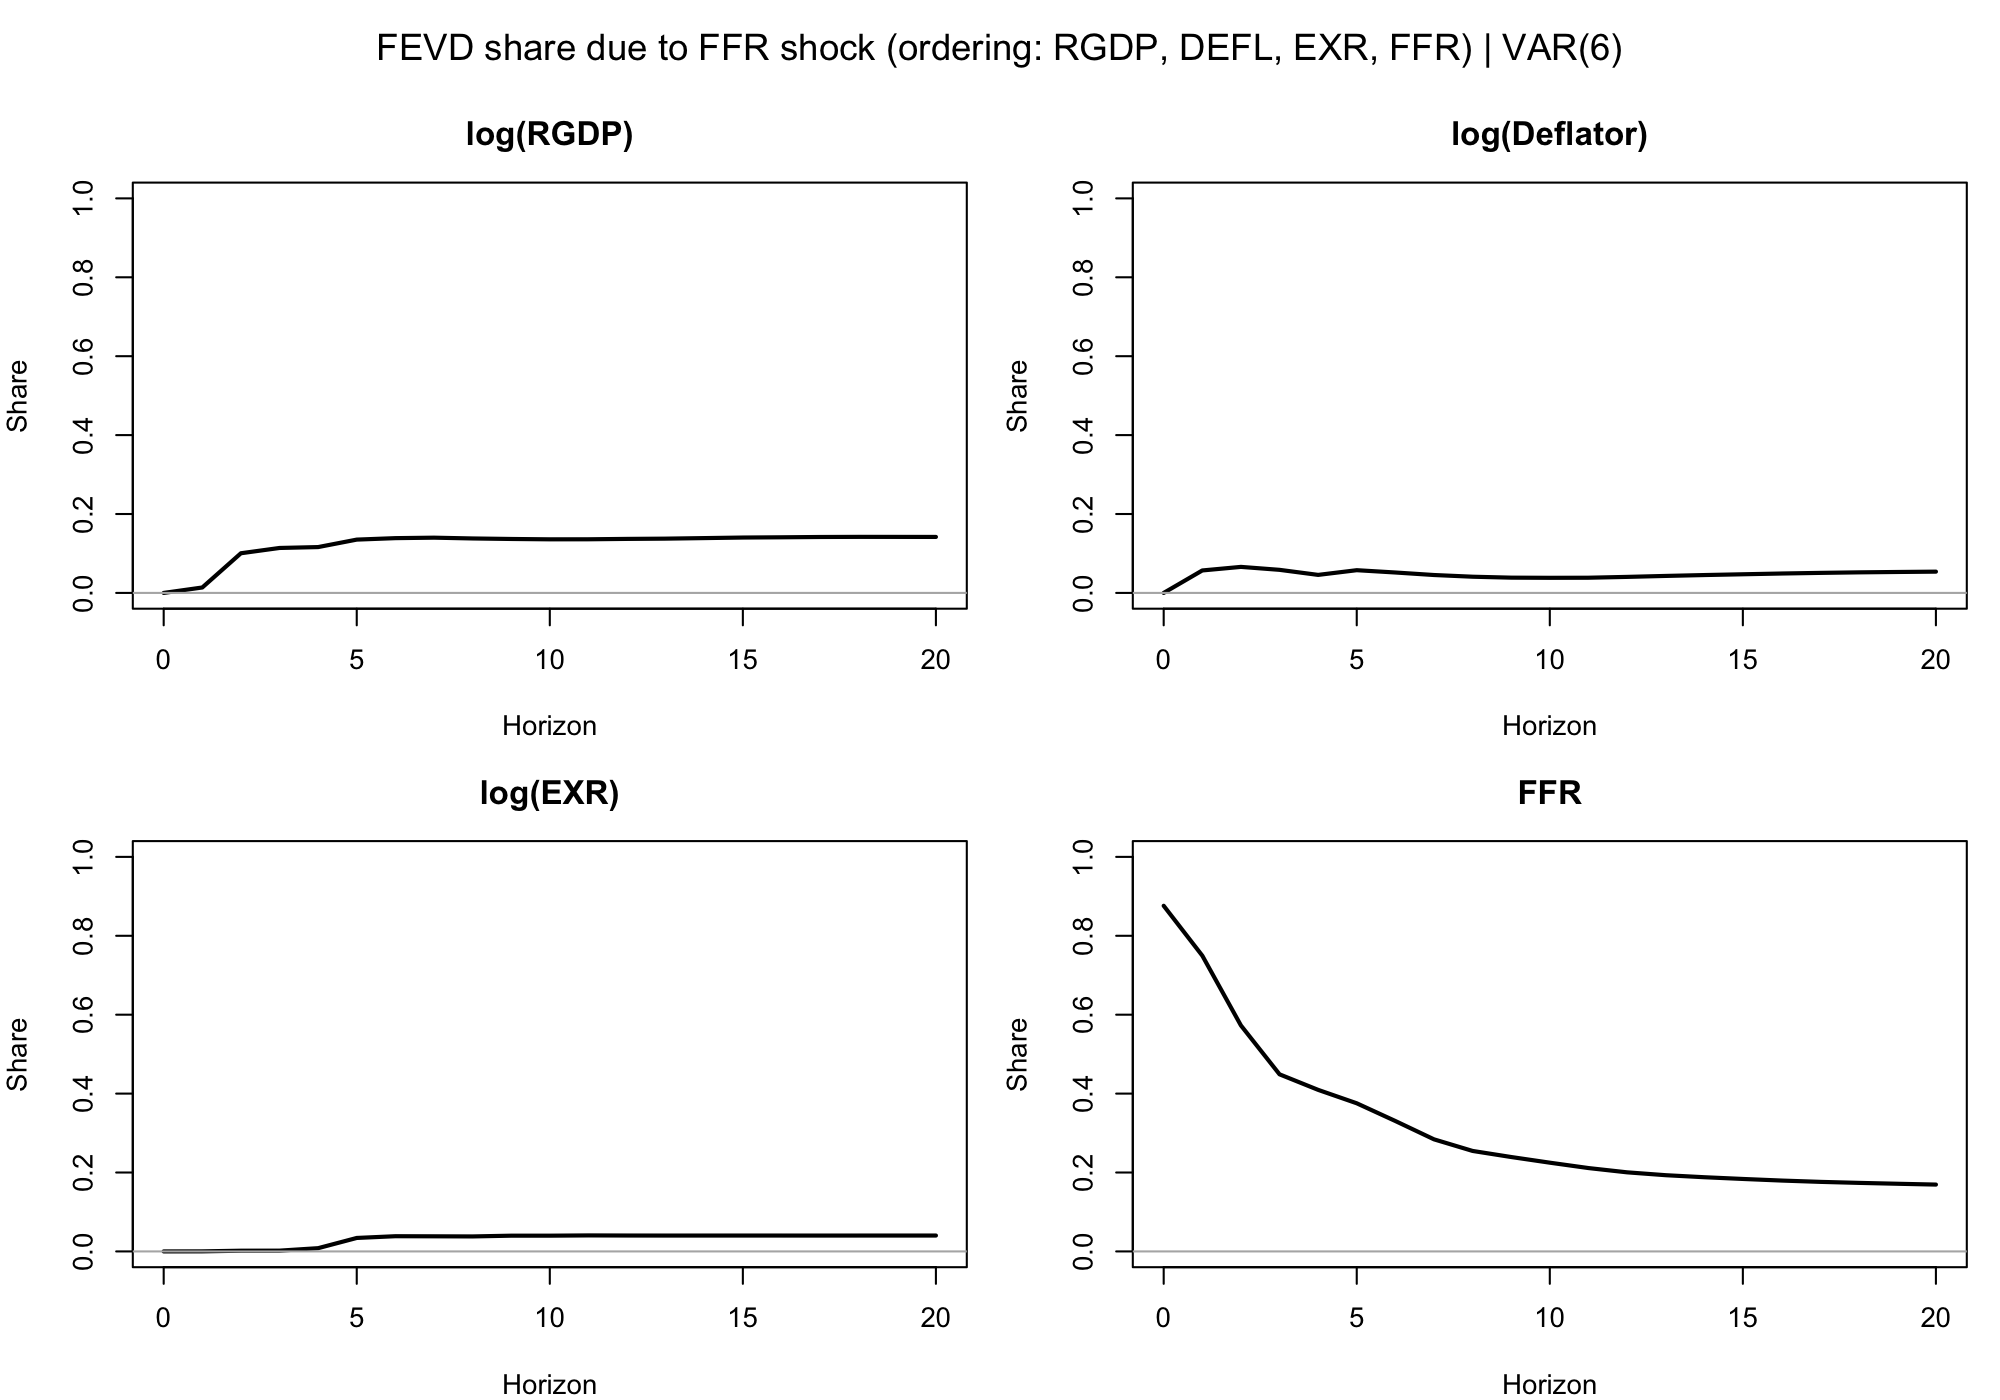
\includegraphics[width=0.6\textwidth]{hw5_fevd_q3_order_ffr_shock.png}
        \caption{FEVD for the $VAR(6)$ model.}
        \label{fig:q3_fevd}
    \end{figure}

    \newpage
    \item The new order results are plotted in Figure \ref{fig:q4_irf}.
    \begin{figure}[htbp]
        \centering
        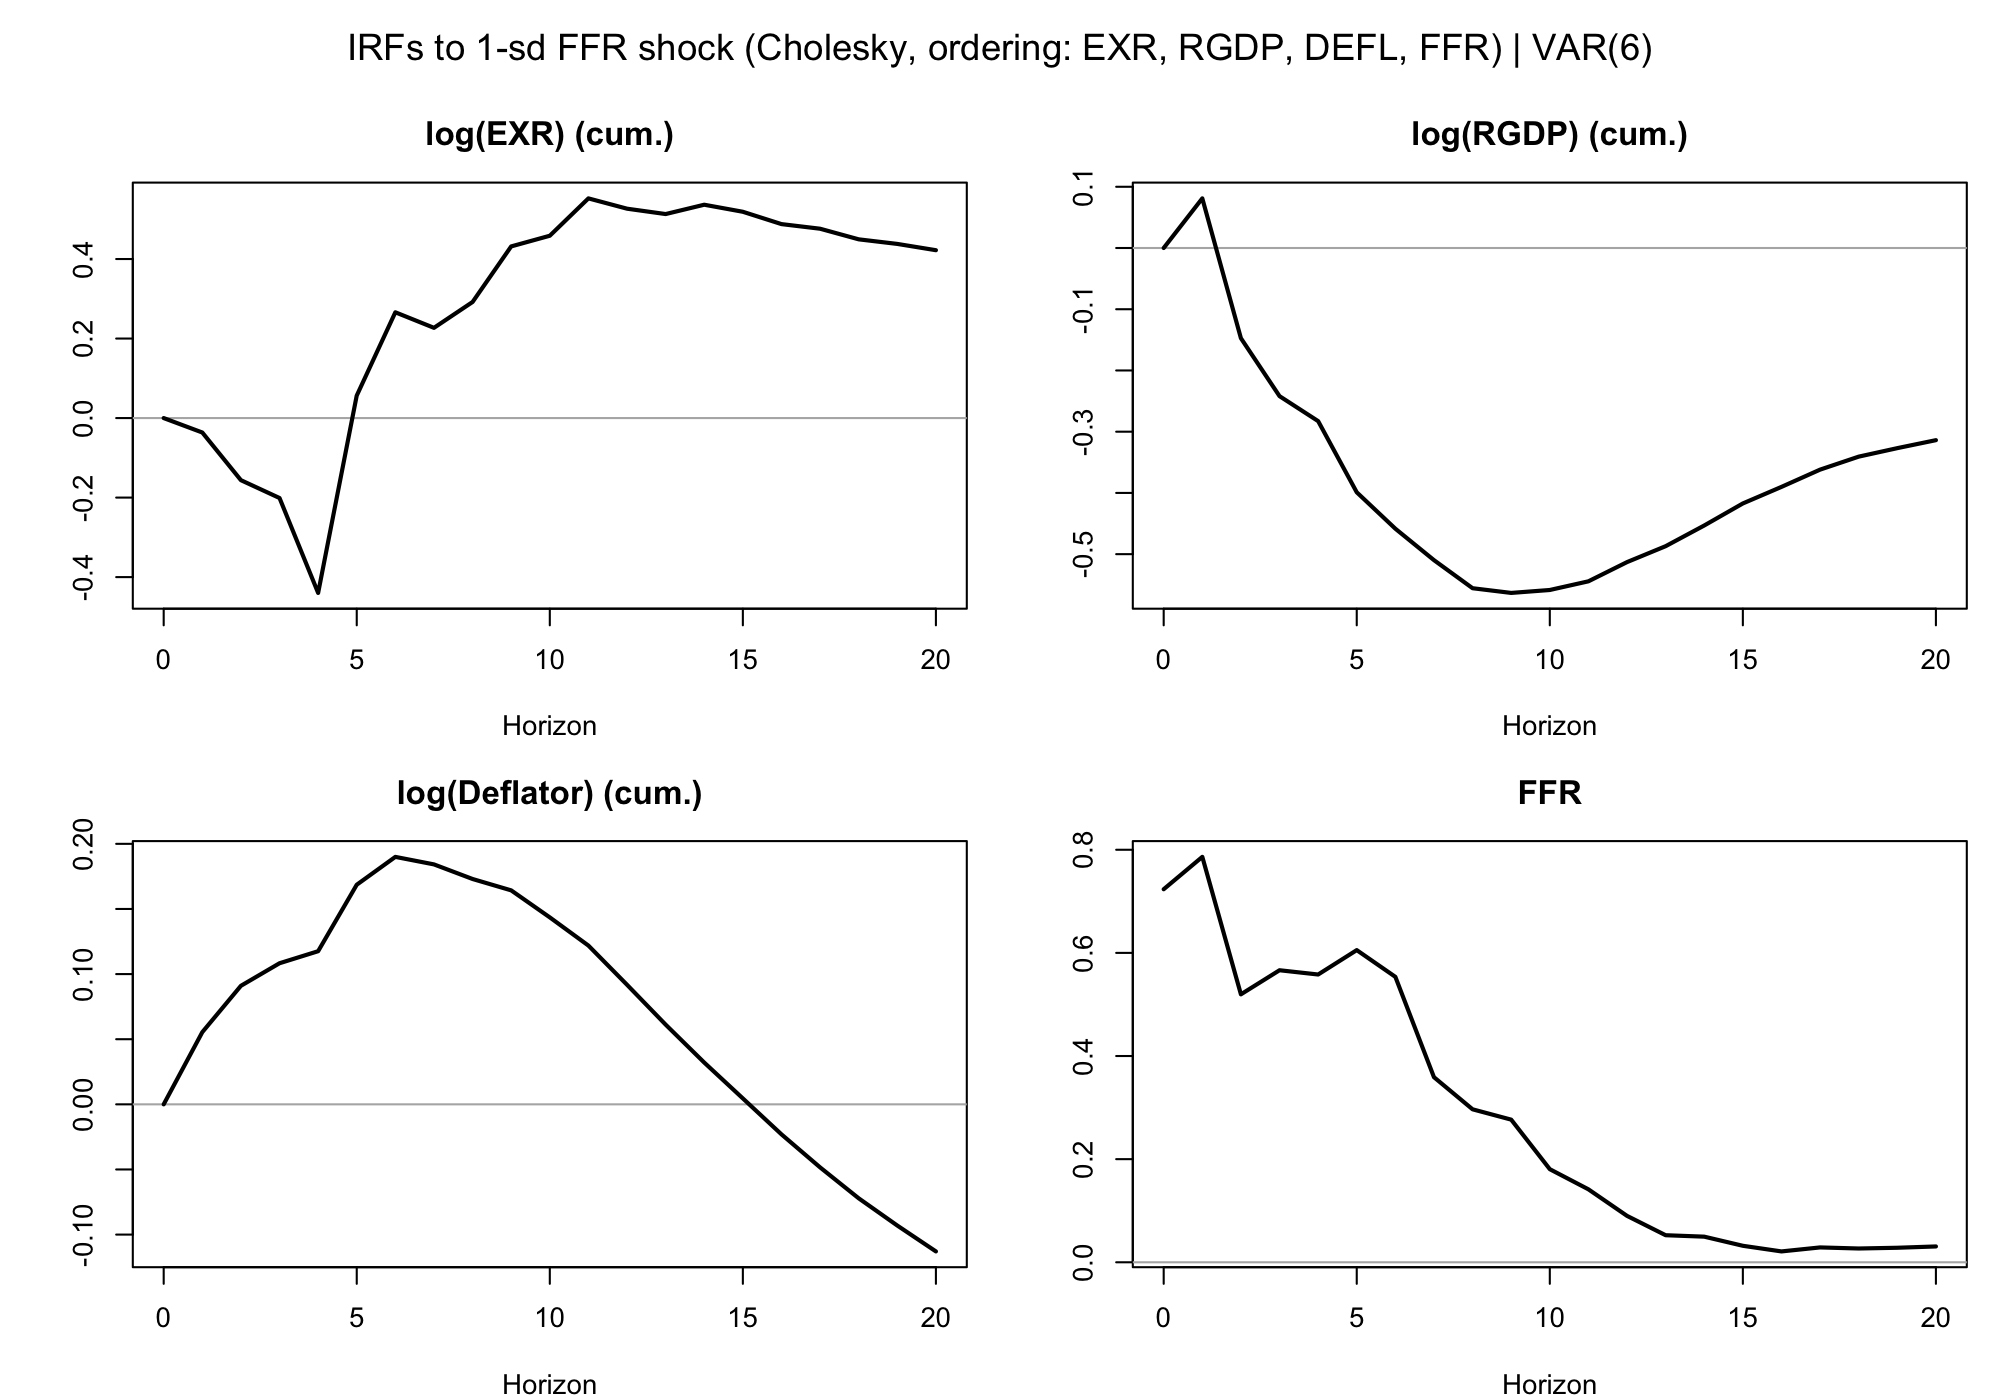
\includegraphics[width=0.6\textwidth]{hw5_irf_q4_order.png}
        \caption{IRF for the $VAR(6)$ model with new order.}
        \label{fig:q4_irf}
    \end{figure}
    
    
\end{enumerate}


\end{document}